\documentclass[tikz,border=8pt]{standalone}
\usepackage{amsmath,amssymb}
\usetikzlibrary{arrows.meta,positioning}
\definecolor{TargetBlue}{HTML}{2364AA}
\definecolor{NuisanceOrange}{HTML}{E6862A}
\definecolor{EfficientGreen}{HTML}{278A64}
\definecolor{NeutralGray}{HTML}{68717C}
\begin{document}
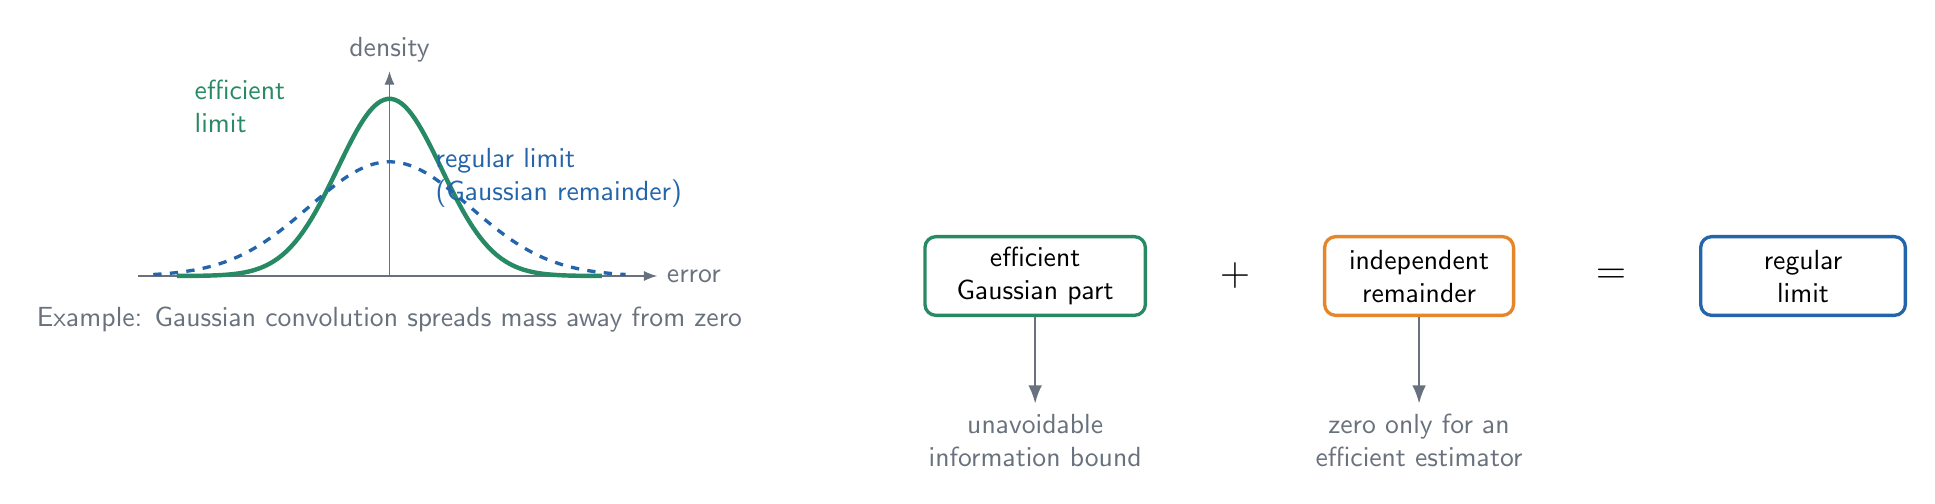
\begin{tikzpicture}[font=\sffamily, >=Latex]
  \begin{scope}
    \draw[->, NeutralGray] (-3.2,0) -- (3.4,0) node[right] {error};
    \draw[->, NeutralGray] (0,0) -- (0,2.6) node[above] {density};
    \draw[EfficientGreen, ultra thick, domain=-2.7:2.7, samples=120, smooth]
      plot (\x,{2.25*exp(-1.15*\x*\x)});
    \draw[TargetBlue, very thick, dashed, domain=-3:3, samples=120, smooth]
      plot (\x,{1.45*exp(-0.48*\x*\x)});
    \node[text=EfficientGreen, align=left] at (-1.9,2.15) {efficient\\limit};
    \node[text=TargetBlue, align=left] at (2.15,1.25)
      {regular limit\\(Gaussian remainder)};
    \node[text=NeutralGray] at (0,-0.55)
      {Example: Gaussian convolution spreads mass away from zero};
  \end{scope}

  \begin{scope}[xshift=8.2cm]
    \node[draw=EfficientGreen, very thick, rounded corners, minimum width=28mm,
      minimum height=10mm, align=center] (e) {efficient\\Gaussian part};
    \node[right=8mm of e, font=\Large] (plus) {$+$};
    \node[draw=NuisanceOrange, very thick, rounded corners, right=8mm of plus,
      minimum width=24mm, minimum height=10mm, align=center] (r) {independent\\remainder};
    \node[right=9mm of r, font=\Large] (equals) {$=$};
    \node[draw=TargetBlue, very thick, rounded corners, right=8mm of equals,
      minimum width=26mm, minimum height=10mm, align=center] (l) {regular\\limit};
    \draw[->, NeutralGray, thick] (e.south) -- ++(0,-1.1)
      node[below, align=center, text=NeutralGray] {unavoidable\\information bound};
    \draw[->, NeutralGray, thick] (r.south) -- ++(0,-1.1)
      node[below, align=center, text=NeutralGray] {zero only for an\\efficient estimator};
  \end{scope}
\end{tikzpicture}
\end{document}
